% !TeX encoding = UTF-8
% !TeX program = pdflatex
% !TeX spellcheck = it_IT

%Pubblico il seguente file per condividere con i miei compagni di corso la struttura da me configurata per la tesi in medicina e chirurgia al Sant'Andrea  

%Qui tutto ciò che c’ è da saper su LaTeX: http://www.lorenzopantieri.net/LaTeX_files/ArteLaTeX.pdf 
%Per scrivere la bibliografia puoi vedere il seguente link: https://www.guitex.org/home/images/doc/GuideGuIT/bibliografia.pdf

\documentclass[a4paper, oneside, noexaminfo]{sapthesis}

%qui ci sono svariati pacchetti utili per far funzionare il programma
\usepackage{microtype}
\usepackage[italian]{babel}
\usepackage[utf8]{inputenc}
\usepackage{imakeidx}
\usepackage{subfigure}
\usepackage[acronym]{glossaries}
\usepackage{graphicx}
\captionsetup{labelsep=quad}
\usepackage{array}
\usepackage{ragged2e}
\usepackage[table]{xcolor}
\usepackage{hyperref}
\usepackage{blindtext}

\usepackage{minted}
\usepackage{pgfplots}
\pgfplotsset{compat=1.7}
\usepackage{wrapfig}

\usepackage{xcolor}
\definecolor{LightGray}{gray}{0.9}

\usepackage[linguistics]{forest} %per dare i diagrammi: https://texdoc.org/serve/forest/0

\newcommand*{\belowrulesepcolor}[1]{% 
  \noalign{% 
  \kern-\belowrulesep \begingroup \color{#1}% 
  \hrule height\belowrulesep \endgroup }%
}
\newcommand*{\aboverulesepcolor}[1]{% 
  \noalign{%
  \begingroup \color{#1}% 
  \hrule height\aboverulesep \endgroup \kern-\aboverulesep }%
}

\usepackage[sort]{natbib}
\bibliographystyle{plainyr-rev} %la bibiografia ordinata in ordine di data dalla più recente
\setcitestyle{super,open={(},close={)}}

\hypersetup{pdftitle={Romito_1932500}, pdfauthor={Romito_1932500}}
\title{Sviluppo di un sistema per rilevare spostamenti in auto tramite il Bluetooth degli smartphone}
\author{Antonio Pietro Romito}
\IDnumber{1932500}
\course{Corso di Laurea in Informatica}
\courseorganizer{Facoltà di Ingegneria dell'Informazione, Informatica e Statistica}
\AcademicYear{2023/2024}
\advisor{Prof. Emanuele Panizzi}
\customadvisorlabel{Relatore}
%\coadvisor{Dott.ssa Nome Cognome}
%\customcoadvisorlabel{Correlatrice}
%\director{Dott.  Nome Cognome}
%\customdirectorlabel{Specializzando\\Responsabile della ricerca}
\authoremail{antormt@gmail.com}
\copyyear{2024}
\thesistype{Relazione di tirocinio}
\examdate{V Sessione A.A. 2023-2024 | Dicembre 2024}

%In caso di titoli di section a 2 righe
%\setlength{\headheight}{22.59052pt}
%\addtolength{\topmargin}{-10.59052pt}

\makeindex

\includeonly{Cap_1,Cap_2,Cap_3,Cap_4,Cap_5,Cap_6}
\newcommand{\Fig}[1]{[{\footnotesize \texttt{Fig.#1}}]}
\newcommand{\citfig}[1]{\ap{\scriptsize\textrm{(\textit{F#1})}}}

\begin{document}
\frontmatter
\maketitle
\dedication{Dedica}

\begin{abstract}
Questa tesi descrive lo sviluppo e l'integrazione di un sensore Bluetooth nell'applicazione GeneroCity, un'applicazione di smart parking progettato dal Gamification Lab della Sapienza Università di Roma. Il sensore è in grado di rilevare automaticamente quando l'utente è alla guida di un'auto, utilizzando interazioni implicite e analisi contestuale dei dati forniti dalla radio Bluetooth degli smartphone, sfruttando le API di Android per la gestione delle connessioni Bluetooth. Il sistema calcola una "confidenza" relativa alla guida, che contribuisce al riconoscimento dello stato dell'utente tramite un algoritmo di media pesata tra vari sensori. I test effettuati hanno dimostrato l'affidabilità del sensore nello scenario reale, confermandone l'efficacia e l'integrazione con il sistema GeneroCity. Futuri sviluppi prevedono l'introduzione di modelli di machine learning per migliorare la determinazione dello stato dell'utente e l'implementazione di servizi esterni per il riconoscimento dei dispositivi Bluetooth.
\end{abstract}
\tableofcontents
%\listoffigures
%\listoftables

\mainmatter
\chapter{Introduzione: GeneroCity, un'Applicazione di SmartParking}

La crescente urbanizzazione e l'aumento del numero di veicoli in circolazione hanno reso la questione della mobilità urbana e della sosta un tema centrale per il futuro delle città. 
Le statistiche presentate dall'Osservatorio AIPARK\footnote{AIPARK - Associazione Italiana Operatori Sosta e Mobilità} nel giugno di quest'anno rivelano una situazione allarmante: l'Italia è al vertice della classifica europea per numero di autovetture, con un rapporto di 690 auto ogni 1.000 abitanti.Questa realtà comporta che circa il 30\% del traffico urbano sia generato da veicoli in cerca di parcheggio, evidenziando un disallineamento tra la domanda di sosta e l'offerta disponibile. Per correggere questo squilibrio è stato calcolato che sarebbe necessario aggiungere 670.000 posti auto, di cui oltre 200 mila solamente a Roma, dove, ad oggi, se ne conta uno ogni 39 residenti.\cite{ref:AIPARK}

Una possibile soluzione a questi problemi è lo \textbf{smart parking}, ossia una strategia che utilizza tecnologie digitali nel tentativo di utilizzare il minor numero di risorse possibili (carburante, tempo, spazio) per ottenere un processo di sosta dei veicoli più veloce, facile e ottimizzato.\cite{ref:smartparking}

\begin{figure}[h]
    \centering
    
\includegraphics[width=0.5\linewidth]{images/gc_logo.png}
    \caption{Logo di GeneroCity}
    \label{fig:gc_logo}
\end{figure}
\section{GeneroCity e il suo scopo}
In questa realtà nasce GeneroCity\cite{ref:generocity}: un’applicazione di smart parking in sviluppo per Android e iOS realizzata dal Gamification Lab del Dipartimento di Informatica della Sapienza Università di Roma. Lo scopo dell'applicazione è quello di facilitare lo scambio dei parcheggi all’interno di un’area urbana puntando sulla generosità degli utenti: la sua idea principale è quella di rilevare quando un utente esce da un parcheggio e segnalarlo agli utenti che ne stanno cercando uno nella stessa zona. Inoltre sono presenti i \textit{GCoins}, ossia una moneta virtuale che gli utenti guadagnano cedendo il loro posto ad altri e possono spendere per prenotarne uno. 
\begin{wrapfigure}{r}{0.5\textwidth}
    \centering
    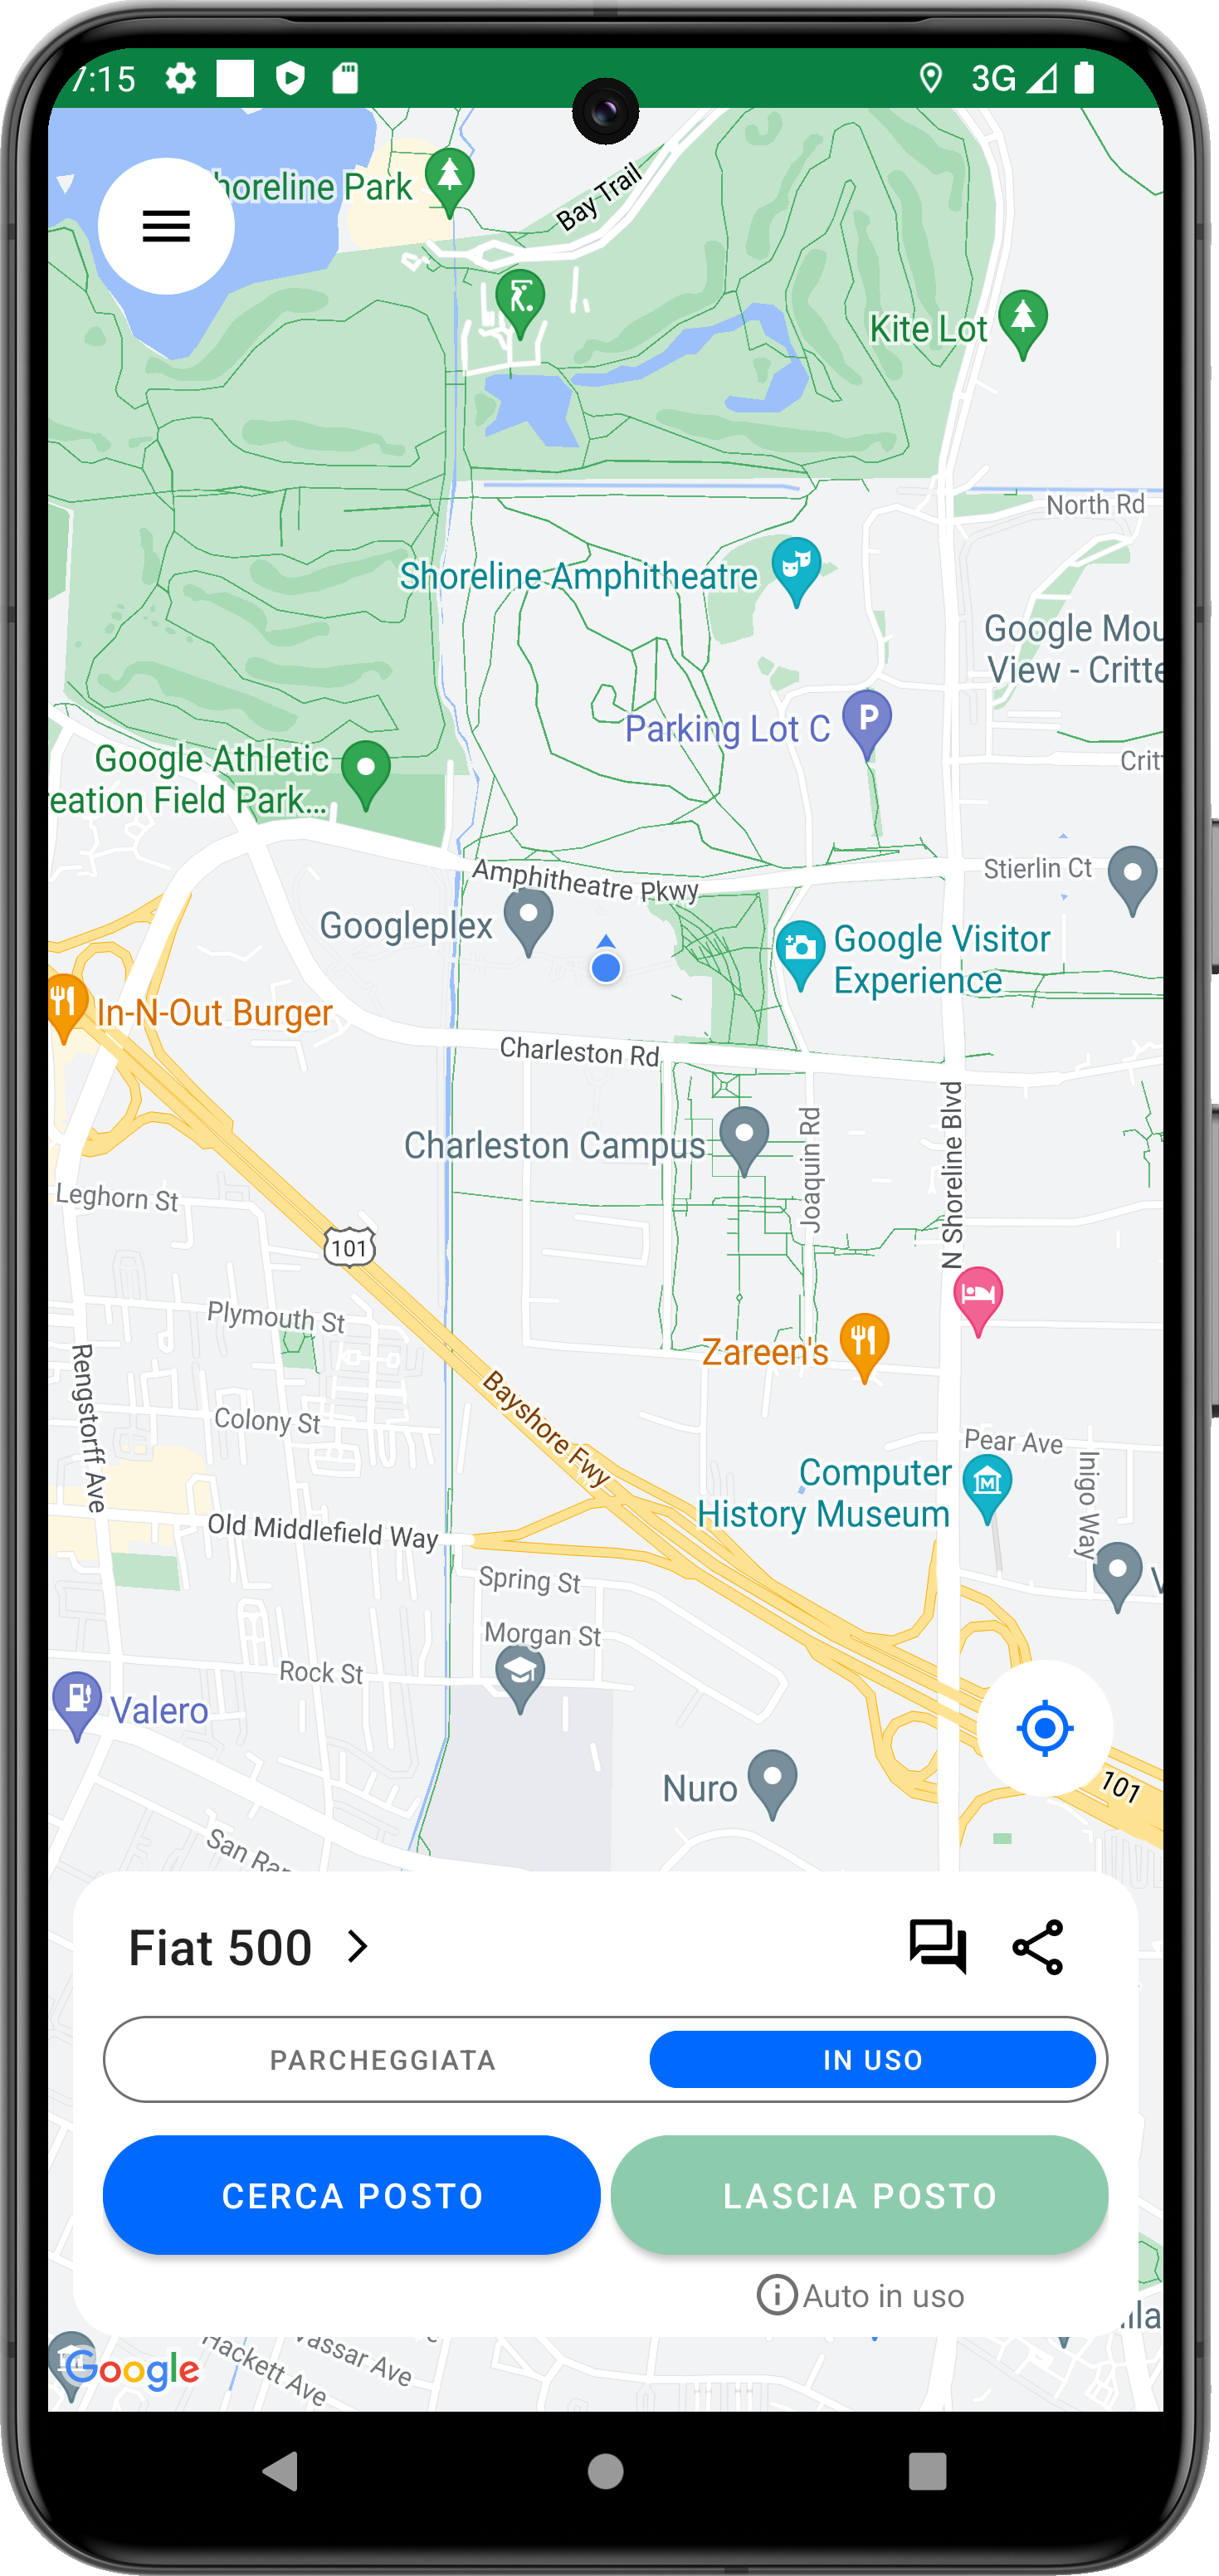
\includegraphics[width=0.9\linewidth]{images/gc_main_activity.png}
    \caption{GeneroCity Android}
    \label{fig:main_screen}
\end{wrapfigure}
Essi rappresentano una componente di gamification\footnote{La gamification è l'utilizzo di elementi mutuati dai giochi e delle tecniche di creazione di giochi in contesti non ludici.} con lo scopo di motivare e coinvolgere gli utenti ad utilizzare l'applicazione.

La vera innovazione introdotta da questo progetto però, è il numero limitato di interazioni: difatti l'applicazione cercherà di prevedere automaticamente quando l'utente lascia o cerca un parcheggio, questo in modo da garantire una maggiore sicurezza alla guida. Il mio ruolo nello sviluppo di GeneroCity è stato quello di utilizzare le funzionalità bluetooth degli smartphone Android per raggiungere tale scopo.

\chapter{L'utilizzo di Android per lo sviluppo del sensore Bluetooth}
\label{chap:app-separata}
Prima di sviluppare il sensore si è scelto di creare una piccola applicazione a sé stante con lo scopo di prendere dimestichezza con l'SDK\footnote{Acronimo che sta per Software Development Kit, ossia un'insieme di strumenti per lo sviluppo del software} di Android per Java, nello specifico con le sue funzionalità riguardanti la connettività via Bluetooth\cite{ref:bluetooth-doc}. Ciò è stato fatto al fine di trovare una strategia efficiente da adottare nello sviluppo del sensore finale
\begin{wrapfigure}[23]{l}{0.4\textwidth}
    \centering
    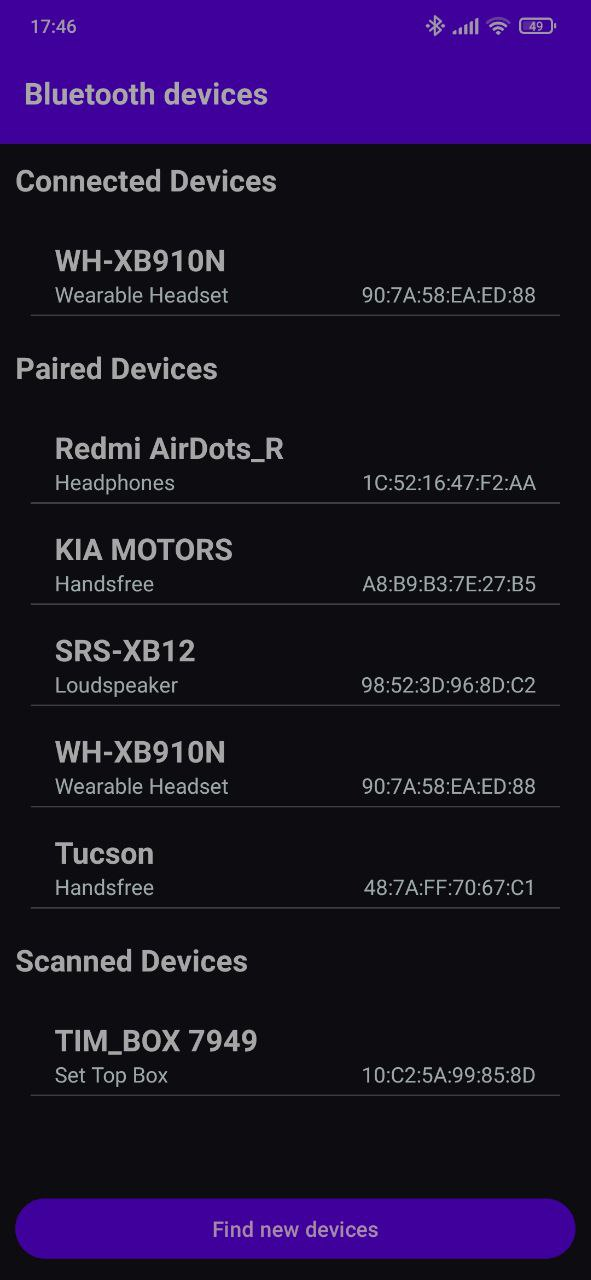
\includegraphics[width=0.9\linewidth]{images/separate_app.png}
    \caption{Interfaccia dell'app}
    \label{fig:separate_app}
\end{wrapfigure}
in GeneroCity, dato che essa contiene molte altre funzionalità e di conseguenza sarebbe stato più difficoltoso effettuare questo tipo di sperimentazione al suo interno. Questa applicazione permette l'esecuzione di tre task, la cui implementazione è stata ritenuta un buon punto di partenza per lo sviluppo del sensore Bluetooth. Esse sono:
\begin{itemize}
    \item la rilevazione del cambiamento dello stato del modulo bluetooth dello smartphone, più specificatamente la sua accensione e lo spegnimento;
    \item l'ottenimento dei dati riguardanti i dispositivi che vengono connessi al Bluetooth;
    \item l'esecuzione di scansioni per trovare dispositivi nelle vicinanze.
\end{itemize}
La scansione dei dispositivi vicini, nonostante sia stata implementata in quest'applicazione, è stata un'idea successivamente scartata nella realizzazione del sensore Bluetooth per due principali motivi: essa, se ripetuta svariate volte, può provocare un eccessivo consumo della batteria e, inoltre, è molto raro che le radio delle macchine si rendano visibili ai dispositivi vicini. Attraverso svariati test è stato notato che tutte le macchine prese in esame erano rilevabili via scansione Bluetooth solamente quando è stata effettuata la procedura per accoppiare\footnote{Con accoppiamento Bluetooth si intende il pairing, ossia il processo in cui due dispositivi Bluetooth effettuano la prima connessione e si scambiano le chiavi di sicurezza, le quali verranno memorizzate per permettere di effettuare rapidamente le connessioni successive.} un nuovo smartphone alla macchina. Di conseguenza non poter trovare le macchine nelle vicinanze attraverso le scansione rende l'utilizzo di questa funzionalità pressoché inutile in GeneroCity. Nonostante ciò ne verrà comunque descritta l'implementazione nel progetto separato.

In questo capitolo verranno quindi illustrati i vari componenti dell'applicazione e come essi implementano le suddette task consentendone la visualizzazione dei risultati. 

\section{I Broadcast Receiver}
Il primo problema che si è presentato nella realizzazione dell'applicazione è stato l'impossibilità di ottenere la lista dei dispositivi connessi al Bluetooth in maniera sincrona tramite le funzionalità messe a disposizione dalle API\footnote{Una API, acronimo di Application Software Interface, è un tipo di interfaccia software che permette ad un programma di offrire servizi e funzionalità ad altri software.} di Android. Infatti il sistema operativo non permette di essere interrogato direttamente dai singoli processi, piuttosto è esso a notificarli quando avvengono degli eventi di sistema, inviando dei messaggi denominati \textit{system broadcast}. Le applicazioni potranno quindi registrarsi per ricevere messaggi relativi ad eventi specifici, ad esempio quando avviene l'accensione e lo spegnimento della modalità aereo il sistema manderà un system broadcast a tutte le app registrate per ricevere questo evento. Questa registrazione avviene attraverso la creazione di oggetti la cui classe estende quella dei \textit{BroadcastReceiver}.\cite{ref:android-broadcast}

La classe sopracitata espone un metodo astratto, denominato \textit{onReceive}, il quale deve essere implementato per definire il comportamento adottato dal programma quando viene ricevuto un system broadcast. Questo metodo ha come parametri il contesto, vale a dire lo stato dell'applicazione al momento in cui è avvenuto, l'evento e l'intent, ossia una rappresentazione dell'evento che ha scaturito la notifica.

\begin{minted}[
framesep=2mm,
linenos,
bgcolor=LightGray,
breaklines
]{java}
public abstract void onReceive(Context context, Intent intent);
\end{minted}

Infine è necessario utilizzare il metodo registerReceiver della classe Context per attuare l'effettiva registrazione al fine di ricevere system broadcast e gestirli attraverso il broadcast receiver passato come parametro. Per far ciò bisogna inoltre dichiarare quali tipologie di eventi esso ascolta, creando un IntentFilter. Viene riportato qui sotto un esempio di codice dove viene registrato un broadcast receiver:
\begin{minted}[
framesep=2mm,
linenos,
bgcolor=LightGray,
breaklines
]{java}
BroadcastReceiver br = new MyBroadcastReceiver();
IntentFilter filter = new IntentFilter(APP_SPECIFIC_BROADCAST);
context.registerReceiver(br, filter);
\end{minted}

Tutti i broadcast receiver definiti si occuperanno solamente di catturare l'evento, sarà poi un metodo astratto, specifico per ognuno di essi, ad essere esteso per implementare l'algoritmo scaturito da esso. Questi metodi saranno estesi direttamente alla creazione dei receiver nella classe Controller, la quale verrà discussa nel paragrafo \ref{ref:controller}. Inoltre tutti i receiver intercettano gli eventi anche quando l'applicazione è in background, pertanto il funzionamento dell'app è inalterato quando essa è in esecuzione ma l'utente non la sta utilizzando direttamente. Di seguito verranno elencati i broadcast receiver implementati e, per ciascuno di essi, verranno discussi i system broadcast che riceveranno e riportato il codice del metodo \textit{onReceive}.

\subsubsection{StatusChangeReceiver}
Esso è il broadcast receiver più semplice ed è stato definito per rilevare l'accensione e lo spegnimento del Bluetooth del dispositivo. Questo receiver si occuperà di intercettare gli eventi che cambiano lo stato della radio Bluetooth, ossia del tipo \textit{BluetoothAdapter.ACTION\_STATE\_CHANGED}.
\begin{minted}[
framesep=2mm,
linenos,
bgcolor=LightGray,
breaklines
]{java}
@Override
public void onReceive(Context context, Intent intent) {
    final String action = intent.getAction();

    if (action != null && action.equals(BluetoothAdapter.ACTION_STATE_CHANGED)) {
        final int state = intent.getIntExtra(BluetoothAdapter.EXTRA_STATE, BluetoothAdapter.ERROR);
        switch (state) {
            case BluetoothAdapter.STATE_OFF:
                onStatusChange(context, false);
                break;
            case BluetoothAdapter.STATE_TURNING_OFF:
                Toast.makeText(context, "Turning bluetooth off...", Toast.LENGTH_SHORT).show();
                break;
            case BluetoothAdapter.STATE_ON:
                onStatusChange(context, true);
                break;
            case BluetoothAdapter.STATE_TURNING_ON:
                Toast.makeText(context, "Turning bluetooth on...", Toast.LENGTH_SHORT).show();
                break;
            default:
                break;
        }
    }
}
\end{minted}

Nel caso in cui il Bluetooth sia stato acceso o spento verrà chiamato il metodo astratto \textit{onStatusChanged}, il quale ha come parametro un booleano che indica lo stato del Bluetooth (true quando è accesso e false se spento). Questo metodo sarà quindi esteso per definire cosa l'applicazione dovrà fare quando ciò avviene.
\begin{minted}[
framesep=2mm,
linenos,
bgcolor=LightGray,
breaklines
]{java}
public abstract void onStatusChange(Context context, boolean bluetoothStatus);
\end{minted}

\subsubsection{FoundDeviceReceiver}
Questo broadcast receiver si occupa di ricevere l'evento riguardante la scoperta di un nuovo dispositivo Bluetooth quando viene effettuata la scansione dei dispositivi nelle vicinanze. Esso verrà notificato degli eventi di tipo \textit{BluetoothDevice.ACTION\_FOUND} e si occuperà di prelevare le informazioni dei dispositivi rilevati attraverso la funzione di utilità \textit{BluetoothDeviceUtils.map}. Essa prende in input il dispositivo Bluetooth e restituisce un oggetto che e ne contiene le informazioni di interesse per l'applicazione (indirizzo MAC, nome del dispositivo e classe bluetooth).
\begin{minted}[
framesep=2mm,
linenos,
bgcolor=LightGray,
breaklines
]{java}
@Override
public void onReceive(Context context, Intent intent) {
    String action = intent.getAction();

    if (action == null 
            || !action.equals(
            android.bluetooth.BluetoothDevice.ACTION_FOUND
        )) {
        return;
    }
    
    android.bluetooth.BluetoothDevice device;
    if (Build.VERSION.SDK_INT >= Build.VERSION_CODES.TIRAMISU) {
        device = intent.getParcelableExtra(
                android.bluetooth.BluetoothDevice.EXTRA_DEVICE,
                android.bluetooth.BluetoothDevice.class
        );
    } else {
        device = intent.getParcelableExtra(
                android.bluetooth.BluetoothDevice.EXTRA_DEVICE
        );
    }
    if (device == null) {
        return;
    }
    
    BluetoothDevice newDevice = BluetoothDeviceUtils.map(device);
    onDeviceFound(newDevice);
}
\end{minted}

Come si può vedere dal codice una volta ottenuti i dati del dispositivo viene chiamato un metodo astratto denominato \textit{onDeviceFound} che verrà esteso per salvare il dispositivo in una struttura dati.
\begin{minted}[
framesep=2mm,
linenos,
bgcolor=LightGray,
breaklines
]{java}
public abstract void onDeviceFound(BluetoothDevice device);
\end{minted}


\subsubsection{ConnectionReceiver}
Gli eventi di tipo \textit{BluetoothDevice.ACTION\_ACL\_CONNECTED} e \textit{BluetoothDevice.ACTION\_ACL\_DISCONNECTED} per ottenere informazioni sui dispositivi che vengono connessi e disconnessi dal Bluetooth saranno gestiti da questo receiver. Quando ciò avviene verrà utilizzata la funzione di mappatura citata precedentemente per prelevarne le informazioni di interesse dai dispositivi.
\begin{minted}[
framesep=2mm,
linenos,
bgcolor=LightGray,
breaklines
]{java}
@Override
public void onReceive(Context context, Intent intent) {
    String action = intent.getAction();

    if (action == null 
        || !action.equals(
            android.bluetooth.BluetoothDevice.ACTION_ACL_CONNECTED
        ) && !action.equals(
            android.bluetooth.BluetoothDevice
                .ACTION_ACL_DISCONNECTED
        )) {
        return;
    }

    android.bluetooth.BluetoothDevice device;
    if (Build.VERSION.SDK_INT >= Build.VERSION_CODES.TIRAMISU) {
        device = intent.getParcelableExtra(
                android.bluetooth.BluetoothDevice.EXTRA_DEVICE,
                android.bluetooth.BluetoothDevice.class
        );
    } else {
        device = intent.getParcelableExtra(
                android.bluetooth.BluetoothDevice.EXTRA_DEVICE
        );
    }

    if (device == null) {
        return;
    }

    BluetoothDevice newDevice = BluetoothDeviceUtils.map(device);

    if (action.equals(android.BluetoothDevice.ACTION_ACL_CONNECTED)) {
        onDeviceConnection(context, newDevice);
    } else {
        onDeviceDisconnection(context, newDevice);
    }
}
\end{minted}

Infine verrà chiamato il metodo astratto \textit{onDeviceConnection} in caso di connessione del dispositivo oppure \textit{onDeviceDisconnection} se si tratta di una disconnessione. Questi metodi verranno estesi per tenere aggiornata una struttura dati che mantiene in memoria i dispositivi connessi via Bluetooth.
\begin{minted}[
framesep=2mm,
linenos,
bgcolor=LightGray,
breaklines
]{java}
public abstract void onDeviceConnection(Context context, BluetoothDevice device);
public abstract void onDeviceDisconnection(Context context, BluetoothDevice device);
\end{minted}

\subsubsection{ImplicitConnectionReceiver}
La creazione di questo receiver deriva dal fatto che tutti quelli descritti precedentemente vengono registrati una volta che viene avviata l'applicazione, pertanto se ci sono già connessi dei dispositivi Bluetooth prima dell'avvio il ConnectionReceiver non è in grado di rilevarli. L'ImplicitConnectionReceiver nasce per risolvere questo problema, difatti esso è una sottoclasse di ConnectionReceiver e funzionerà anche quando l'applicazione è completamente chiusa: esso viene registrato nel manifest\footnote{Il manifest Android è un file che definisce la struttura, le funzionalità e i requisiti di un'applicazione Android.} dell'applicazione e sarà quindi il sistema operativo a "svegliarla" se essa non è in esecuzione, così da permettere l'esecuzione di codice in risposta ad una connessione o disconnessione di un dispositivo Bluetooth. Segue la porzione di manifest dove viene dichiarato il receiver specificandone gli intent per cui esso sarà notificato.
\begin{minted}[
framesep=2mm,
linenos,
bgcolor=LightGray,
breaklines
]{xml}
<receiver 
    android:name="receivers.ImplicitConnectionReceiver"
    android:exported="true">
    <intent-filter>
        <action 
            android:name= "android.bluetooth.device.action.ACL_CONNECTED"/>
        <action
            android:name= "android.bluetooth.device.action.ACL_DISCONNECTED"/>
    </intent-filter>
</receiver>
\end{minted}

Esso essendo di tipo ConnectionReceiver eredita anche il metodo onReceive di quest'ultimo, tuttavia deve fornire un implementazione dei suoi metodi astratti. Nel caso della connessione di un dispositivo il metodo \textit{onDeviceConnection} si occuperà di caricare un'insieme dei dispositivi connessi in quel momento da un file, aggiungere il dispositivo connesso in quel momento e salvare l'insieme aggiornato sul file.
\begin{minted}[
framesep=2mm,
linenos,
bgcolor=LightGray,
breaklines
]{java}
@Override
public void onDeviceConnection(Context context, BluetoothDevice device) {
    Set<BluetoothDevice> connectedDevices = loadConnectedDevices(context);
    connectedDevices.add(device);
    saveConnectedDevices(context, connectedDevices);
}
\end{minted}

Per quando riguarda il metodo \textit{onDeviceDisconnection} viene fatta pressoché la medesima cosa: viene caricato l'insieme dei dispositivi, rimosso il dispositivo disconnesso e salvato l'insieme aggiornato.
\begin{minted}[
framesep=2mm,
linenos,
bgcolor=LightGray,
breaklines
]{java}
@Override
public void onDeviceDisconnection(Context context, BluetoothDevice device) {
    Set<BluetoothDevice> connectedDevices = loadConnectedDevices(context);
    connectedDevices.remove(device);
    saveConnectedDevices(context, connectedDevices);
}
\end{minted}

Grazie a questo receiver il Controller, non appena verrà istanziato all'avvio dell'applicazione, potrà ottenere i dispositivi connessi precedentemente l'avvio in quanto verranno caricati dal file da esso aggiornato.

\section{Il Controller} \label{ref:controller}
Il Controller è l'unità centrale dell'applicazione infatti esso si occupa di mantenere gli insiemi dei dispositivi Bluetooth accoppiati al telefono, quelli rilevati dalle scansioni e infine i dispositivi connessi. Esso implementa due design pattern\footnote{Un design pattern, traducibile in schema di progettazione, nell'ambito dell'ingegneria del software è una soluzione generale ad un problema ricorrente.}: il \textbf{singleton pattern}, il quale consente alla classe Controller di avere un'unica istanza accessibile da qualunque punto del codice, e l'\textbf{observer pattern} che permette ad a altri oggetti di registrarsi per venire notificati dal Controller quando esso cambia il suo stato. In particolare lo stato del Controller è rappresentato da i suoi seguenti attributi:
\begin{itemize}
    \item \textit{isBluetoothEnabled}, un flag che indica se il modulo Bluetooth del dispositivo è acceso o spento;
    \item \textit{pairedDevices}, l'insieme dei dispositivi Bluetooth accoppiati allo smartphone;
    \item \textit{scannedDevices}, l'insieme dei dispositivi Bluetooth trovati durante l'ultima scansione;
    \item \textit{connectedDevices}, l'insieme dei dispositivi Bluetooth connessi allo smartphone.
\end{itemize}

Inoltre è presente una lista di listener, ossia degli oggetti che verranno notificati dal Controller ogni qualvolta esso cambierà stato. Nello specifico si tratta di una lista di \textit{Runnable}, ossia un'interfaccia funzionale\footnote{In Java un'interfaccia funzionale è un'interfaccia che contiene un solo metodo astratto. Esse permettono di utilizzare il paradigma di programmazione funzionale, facendo in modo di rappresentare delle funzioni come oggetti e potendole quindi passare come parametri ad altre funzioni.} il cui metodo non prende input né produce output ma esegue semplicemente una sequenza di istruzioni. Essi verranno eseguiti sequenzialmente uno dopo l'altro ogni volta che verrà chiamato il metodo \textit{notifyListener}, cosa che avverrà ad ogni cambiamento di stato del Controller.

Come detto in precedenza il Controller utilizza i broadcast receiver sopra descritti in modo da poter aggiornare il suo stato in risposta agli eventi di sistema. Tutti i receiver verranno creati come costanti della classe Controller e saranno registrati nel suo costruttore. Nello specifico vengono estese in maniera anonima le loro classi in modo da fornire un'implementazione dei metodi astratti. Di seguito verrà descritto come gli aggiornamenti di stato avvengono attraverso questi metodi.

\subsubsection{Stato del modulo Bluetooth (accensione e spegnimento)}
Per rilevare l'accensione e lo spegnimento del Bluetooth dello smartphone il Controller crea uno StatusChangeReceiver fornendo un'implementazione del metodo onStatusChange. Esso ha il compito di assegnare il nuovo valore al flag isBluetoothEnabled del controller sulla base del parametro booleano bluetoothStatus, il quale sarà true se il bluetooth è acceso o false altrimenti. In caso di spegnimento, verrà svuotato l'insieme dei dispositivi connessi. Infine verranno notificati i listener del cambiamento.
\begin{minted}[
framesep=2mm,
linenos,
bgcolor=LightGray,
breaklines
]{java}
private final StatusChangeReceiver statusChangeReceiver = new StatusChangeReceiver() {

        @Override
        public void onStatusChange(Context context, boolean bluetoothStatus) {
            isBluetoothEnabled = bluetoothStatus;
            if (!bluetoothStatus) {
                connectedDevices.clear();
            }
            notifyListeners();
        }
};
\end{minted}

\subsubsection{Connessione e disconnessione di un dispositivo}
Allo stesso modo verrà creato un ConnectionReceiver per aggiornare l'insieme dei dispositivi connessi quando uno di essi si connette o disconnette. Vengono quindi implementati i metodi onDeviceConnection e onDeviceDisconnection per far ciò: nel primo viene aggiunto il dispositivo ottenuto all'insieme dei dispositivi connessi mentre nel secondo il dispositivo viene rimosso. In entrambi i casi vengono notificati i listener.
\begin{minted}[
framesep=2mm,
linenos,
bgcolor=LightGray,
breaklines
]{java}
private final ConnectionReceiver connectionReceiver = new ConnectionReceiver() {

    @Override
    public void onDeviceConnection(Context context, BluetoothDevice device) {
        connectedDevices.add(device);
        notifyListeners();
    }

    @Override
    public void onDeviceDisconnection(Context context, BluetoothDevice device) {
        connectedDevices.remove(device);
        notifyListeners();
    }
};
\end{minted}

\subsubsection{Scoperta di un nuovo dispositivo durante la scansione}
Quando invece verrà effettuata la scansione dei dispositivi Bluetooth nelle vicinanze sarà il FoundDeviceReceiver a essere notificato ogni volta che ne viene trovato uno. Viene infatti implementato il suo metodo onDeviceFound per aggiungere il dispositivo all'insieme dei dispositivi trovati tramite la scansione e successivamente vengono notificati i listener del controller.
\begin{minted}[
framesep=2mm,
linenos,
bgcolor=LightGray,
breaklines
]{java}
private FoundDeviceReceiver foundDeviceReceiver = new FoundDeviceReceiver() {

    @Override
    public void onDeviceFound(BluetoothDevice device) {
        scannedDevices.add(newDevice);
        notifyListeners();
    }
};
\end{minted}

\section{La presentazione dei dati}
L'ultimo componente di quest'applicazione è l'interfaccia utente che permetterà la visualizzazione dispositivi amministrati dal Controller e di far partire le scansioni Bluetooth attraverso un bottone. Essa mostrerà i dispositivi divisi in tre elenchi differenti: uno per i dispositivi connessi, uno per quelli accoppiati e infine uno per quelli trovati via scansione. Queste liste sono amministrate da tre oggetti diversi tutti appartenenti alla classe \textit{BluetoothDeviceAdapter}, la quale si occupa di convertire gli elementi di una lista di dispositivi in una componente grafica che ne riporta le relative informazioni, come visibile in figura \ref{fig:separate_app}.
Inoltre in questa classe è presente un metodo astratto, denominato \textit{updateDevices}, che si occupa di aggiornare la lista dei dispositivi dell'adapter:
\begin{minted}[
framesep=2mm,
linenos,
bgcolor=LightGray,
breaklines
]{java}
public abstract void updateDevices();
\end{minted}
Esso sarà implementato alla creazione dei vari BluetoothDeviceAdapter in modo da ottenere dal Controller la lista dei dispositivi utili per l'adapter e successivamente notificarlo del cambiamento, così facendo esso renderizzerà nuovamente i suoi componenti grafici con i nuovi dati. Poiché l'implementazione è pressoché uguale per tutti gli adapter, si riporta come esempio solamente il codice di quello utilizzato per aggiornare i dispositivi connessi:
\begin{minted}[
framesep=2mm,
linenos,
bgcolor=LightGray,
breaklines
]{java}
BluetoothDeviceAdapter connectedDeviceAdapter = new BluetoothDeviceAdapter(this) {
    @Override
    public void updateDevices() {
        BluetoothController controller = BluetoothController
            .getInstance(MainActivity.this);
        devices = controller.getConnectedDevices();
        notifyDataSetChanged();
    }
};
\end{minted}
L'unica differenza che avranno gli altri BluetoothDevice adapter è quale lista di dispositivi essi richiederanno al Controller: per ottenere la lista aggiornata l'adapter che si occupa dei dispositivi accoppiati userà il metodo \textit{getPairedDevices} del Controller, quello che si occupa dei dispositivi scansionati \textit{getScannedDevices}, mentre, come visto sopra, quello relativo ai dispositivi connessi \textit{getConnectedDevices}.

Infine i metodi updateDevices di ogni BluetoothDeviceAdapter saranno registrati come listener del Controller. In tal modo ogni qual volta viene aggiornato lo stato di quest'ultimo e verranno notificati i listener questi metodi saranno eseguiti così da avere un riscontro grafico dell'aggiornamento avvenuto.
\begin{minted}[
framesep=2mm,
linenos,
bgcolor=LightGray,
breaklines
]{java}
controller.addListener(pairedDeviceAdapter::updateDevices);
controller.addListener(scannedDeviceAdapter::updateDevices);
controller.addListener(connectedDeviceAdapter::updateDevices);
\end{minted}

Ora che sono stati definiti tutti i componenti si può fornire un esempio del flusso di aggiornamento dell'applicazione, nello specifico esso verrà descritto in seguito alla connessione di un dispositivo Bluetooth: quando ciò accade il ConnectionReceiver viene notificato il quale esegue il metodo onDeviceConnection, che si occupa di aggiungere il dispositivo all'insieme dei dispositivi connessi del Controller. Una volta fatto ciò, a seguito del cambiamento di stato, verranno eseguiti sequenzialmente tutti i listener registrati. Tra di essi è presente il metodo updateDevices del connectedDeviceAdapter il quale interrogherà il Controller per ottenere la lista aggiornata dei dispositivi connessi e farà partire la procedura di rendering grafico della lista utilizzando i nuovi dati ottenuti. In maniera equivalente ciò avverrà per tutte le altre liste quando accade un evento che aggiorna uno degli insiemi dei dispositivi ed invece, per quanto riguarda il cambiamento di stato del modulo Bluetooth del telefono, se il Bluetooth viene spento le liste saranno rimpiazzate da un messaggio che intima l'utente di accenderlo e saranno nuovamente mostrate quando esso viene acceso. 

\section{Testing}
A pari passo con lo sviluppo di questa applicazione è stato verificato il suo funzionamento su più smartphone e, al termine di esso, è stato possibile rilevare le connessione di dispositivi Bluetooth, sia con l'applicazione in foreground che in background, ed effettuare scansioni per trovarne di nuovi, il tutto con successo e senza incorrere in alcun tipo di errore. A questo punto si è potuto procedere con l'implementazione del sensore Bluetooth andando ad integrare in GeneroCity un sistema basato su quanto progettato per quest'applicazione

Nel prossimo capitolo verrà illustrata Generocity e in particolare il suo sistema di sensori per poi descrivere, nel capitolo \ref{chap:Bluetooth-sensor}, l'integrazione del nuovo sensore Bluetooth.
\chapter{I Sensori e il loro utilizzo per ottenere Interazioni Implicite}
Come detto in precedenza una delle funzionalità principali dell'applicazione è riconoscere come l'utente si sta spostando in un determinato momento. In questa fase dello sviluppo ci siamo concentrati nello specifico nel dedurre se un'utente si trova alla guida o meno. Di seguito si spiegherà come questo scopo è stato raggiunto attraverso il lavoro coordinato di vari sensori.
\section{I sensori}
In GeneroCity un sensore è un modulo software che analizza il contesto in cui si trova l'utente in uno specifico istante per determinare l'azione compiuta da quest'ultimo. In particolare ciascuno di essi calcola un valore reale compreso tra 0 e 1, detto \textbf{confidenza}, il quale rappresenta il grado di sicurezza con il quale il sensore ha effettuato la rilevazione (dove 0 rappresenta una sicurezza minima e 1 massima). Dato che nella versione attuale dell'applicazione l'azione che viene rilevata solamente una, possiamo approssimare la confidenza come la probabilità che l'utente stia guidando dove:
\begin{itemize}
    \item un valore compreso tra 0 e 0,5 (stato \textit{walking}) indica che l'utente non sta guidando;
    \item il valore 0,5 (stato \textit{unknown}) denota che il sensore non è in grado di inferire lo stato dell'utente;
    \item una confidenza compresa tra 0,5 e 1 (stato \textit{automotive}) segnala che l'utente sta guidando.
\end{itemize}

Per analizzare il contesto e calcolare la confidenza ogni sensore si può basare sulle rilevazioni di un vero e proprio sensore (come quelli di movimento o ambientali), sullo stato di una specifica componente del dispositivo, ad esempio la batteria, oppure può utilizzare la connettività (ad esempio Wi-Fi o Bluetooth) o altre tecnologie e protocolli specifici, come la geolocalizzazione attraverso GPS. Una linea guida importante per lo sviluppo di un sensore è che esso faccia uso una sola di queste tecnologie per effettuare la sua computazione, in modo che siano tutti indipendenti tra di loro, di modo che sarà poi l'insieme dei risultati ottenuti da tutti i sensori in uno specifico lasso di tempo a concorrere al calcolo della confidenza finale. Questo valore sarà poi quello che effettivamente indicherà se l'utente sta guidando o meno.

\section{Il flusso di aggiornamento della confidenza in GeneroCity Android}

\subsection{L'interfaccia Sensor}
\subsection{L'invio di dati al server}
\subsection{Il compito del sensore Bluetooth}
L'obbiettivo del mio tirocinio: sviluppare un sensore per capire se l'utente sta guidando basandosi sui dispositivi connessi al bluetooth
Scelta di implementarlo prima in un progetto separato, motivazioni:
\begin{itemize}
    \item prendere dimestichezza con l'SDK di Android
    \item imparare ad utilizzare le API di Android per la connettività via bluetooth per
    \begin{itemize}
        \item rilevare l'accensione e lo spegnimento del bluetooth stesso
        \item ottenere i dati dei dispositivi connessi
        \item effettuare scansioni per trovare dispositivi vicini
    \end{itemize}
\end{itemize}

\chapter{Integrazione del sensore bluetooth in Generocity} \label{chap:Bluetooth-sensor}
In questo capitolo verrà spiegato come è stato integrato il sensore Bluetooth nel sistema precedentemente descritto. Esso si basa sulla struttura illustrata nel capitolo \ref{chap:app-separata} a cui verranno aggiunti degli algoritmi per rilevare la connessione di automobili e per il calcolo della confidenza. Tutti i file riguardanti il nuovo sensore sono stati aggiunti in un package\footnote{In Java un package è una sorta di contenitore che ha lo scopo di raggruppare classi, interfacce ed enumerazioni logicamente correlate.}, denominato \textit{it.uniroma1.di.generocity.sensors.bluetooth}, il quale a sua volta è all'interno di \textit{it.uniroma1.di.generocity.sensors} che raccoglie tutto il codice sorgente relativo a tutti i sensori. I suddetti file sono poi stati organizzati a loro volta nei package qui riportati:
\begin{itemize}
    \item \textit{presentation}, il quale contiene tutte le classi utili alla presentazione dei dati e all'interfaccia utente;
    \item \textit{receivers}, al cui interno sono definiti tutti i broadcast receiver utilizzati;
    \item \textit{utils}, che contiene una classe di utilità e delle classi utilizzate per rappresentare i dispositivi Bluetooth sotto forma di oggetti.
\end{itemize}
Inoltre direttamente in \textit{it.uniroma1.di.generocity.sensors.bluetooth} sono presenti due classi: il Controller, che, pur mantenendo il suo scopo descritto nel capitolo \ref{chap:app-separata}, è stato leggermente modificato, e la classe BluetoothSensor, la quale fungerà da interfaccia tra il Controller ed il modulo dei sensori calcolando e aggiornando la confidenza del sensore Bluetooth.

\section{Le modifiche attuate al Controller}
Come per l'applicazione sviluppata precedentemente, il Controller assume un ruolo centrale per il sensore Bluetooth, difatti è qui che verrà mantenuto lo stato del sensore. Allo stesso modo in esso è presente una lista di listener che verranno notificati ad ogni cambiamento di stato. Quest'ultimo è rappresentato dai seguenti attributi:
\begin{itemize}
    \item \textit{isBluetoothEnabled}, un flag che, come nell'applicazione separata, indica se il Bluetooth è acceso o spento;
    \item \textit{cars}, una mappa che mantiene i dati dei dispositivi Bluetooth delle ultime 10 macchine connesse allo smartphone;
    \item \textit{connectedDevices}, l'insieme dei dispositivi connessi.
\end{itemize}
A differenza del primo Controller descritto non sono presenti gli insiemi riguardanti i dispositivi accoppiati e quelli rilevati durante le scansioni, in quanto, come detto in precedenza, l'idea di effettuare la scansione dei dispositivi nelle vicinanze è stata scartata. Per quanto riguarda l'insieme dei dispositivi accoppiati si è scelto di sostituirlo con la mappa cars, così da mantenere in memoria solo i dispositivi connessi precedentemente rilevati come macchine, il tutto per accelerare il processo di rilevamento di un'automobile come verrà descritto nel paragrafo \ref{ref:rilevamento_macchina}. Questa mappa associa l'indirizzo MAC\footnote{L'indirizzo MAC è in codice di 48 bit associato univocamente ad ogni dispositivo di rete.} del dispositivo all'oggetto contenente le sue relative informazioni e consente la memorizzazione di dieci dispositivi al massimo, rimpiazzando quello connesso meno recentemente in caso si provasse ad inserirne un undicesimo. Inoltre la mappa viene salvata nella memoria dello smartphone attraverso le SharedPreferences\footnote{Un oggetto di tipo SharedPreferences punta ad un file contenente coppie chiave-valore e fornisce dei metodi per scrivere e leggere quest'ultimo.} in modo da renderla persistente in memoria anche dopo la chiusura dell'app.

Infine il Controller, come il suo corrispondente nell'altra applicazione, utilizza i broadcast receiver per ascoltare gli eventi di sistema e aggiornare il suo stato di conseguenza. Esso registra uno StatusChangeReceiver esattamente come descritto nel paragrafo \ref{ref:controller} in modo da rilevare l'accensione e lo spegnimento del Bluetooth. A differenza di questo receiver, il ConnectionReceiver invece è stato leggermente modificato per permettere di verificare se i dispositivi connessi sono macchine o meno, mantenendo la sua normale funzione di inserire questi dispositivi nell'insieme dei dispositivi connessi e rimuoverli da esso quando si disconnettono. L'ultimo broadcast receiver implementato è l'ImplicitConnectionReceiver anche esso senza modifiche, il Controller però, al momento della sua creazione, non caricherà solamente i dispositivi connessi dal file, ma, per ognuno di essi eseguirà l'algoritmo per verificare se si tratta di un'automobile. I dettagli di questo algoritmo saranno discussi nel prossimo paragrafo. L'unico broadcast receiver non presente nel nuovo controller è il FoundDeviceReceiver in quanto il suo utilizzo è limitato alle scansioni Bluetooth.

\subsection{L'algoritmo per l'identificazione di automobili}\label{ref:rilevamento_macchina}
Come detto in precedenza, quando viene connesso un dispositivo viene attuata una procedura per verificare se si tratta del Bluetooth di un'autoradio o di altoparlanti di una macchina. Tale procedura è implementata nel metodo \textit{onDeviceConnection} del ConnectionReceiver che, allo stesso modo dell'app sviluppata precedentemente, si occupa di rilevare le connessioni dei dispositivi Bluetooth. Viene qui riportato il codice del metodo:
\begin{minted}[
framesep=2mm,
linenos,
bgcolor=LightGray,
breaklines
]{java}
@Override
public void onDeviceConnection(Context context, BluetoothDevice device) {
    BluetoothDevice car = getCar(device.getMacAddress());
    if (car != null) {
        device = car;
    } else {
        device.checkIfCar();
    }

    if (device.isCar()) {
        device.saveConnection();
        BluetoothController.this.saveCar(context, device);
    }

    connectedDevices.add(device);
    notifyListeners();
}
\end{minted}
Come prima cosa il metodo cerca di ottenere dalla mappa \textit{cars} il dispositivo connesso e, nel caso esso non sia presente nella struttura dati, verrà utilizzato il metodo \textit{checkIfCar} della classe dei dispositivi Bluetooth, il quale effettua il vero e proprio controllo al fine di determinare se si tratta di un'auto o meno. Nel caso in cui il dispositivo connesso è un'automobile, a prescindere se fosse già salvata o meno, viene chiamato un metodo denominato \textit{saveConnection}, il quale si occupa di aggiornare il numero di connessioni effettuate da quel dispositivo e la data e ora della sua ultima connessione. Successivamente verrà salvata l'auto nella mappa in modo da aggiungere il dispositivo o aggiornare i suoi dati se già presente. Infine verrà aggiunto il dispositivo nell'insieme dei dispositivi connessi e verranno notificati i listener del Controller. Di seguito viene riportato il diagramma di flusso che descrive le istruzioni eseguite al momento della connessione di un nuovo dispositivo.

\begin{figure}[H]
    \centering
    \caption{Diagramma di flusso del metodo onDeviceConnection}
    \label{fig:onDeviceConnection}
    
    \begin{tikzpicture}[node distance=2cm]
        \node (start) [startstop] {\textbf{Inizio}};
        \node (in1) [io, below of=start] {\textbf{Input:} dispositivo};
        \node (dec1) [decision, below of=in1, yshift=-1cm] {dispositivo è presente in \textit{cars}?};
        \node (pro1) [process, below of=dec1, xshift=-4cm, yshift=-1cm] {prende il dispositivo con lo stesso mac da \textit{cars}};
        \node (pro2) [process, below of=dec1, xshift=4cm, yshift=-1cm] {controlla se il dispositivo è un'auto con \textit{chekIfCar}};
        \node (dec2) [decision, below of=dec1, yshift=-4cm] {dispositivo è un'auto?};
        \node (pro3) [process, below of=dec2, xshift=-4cm, yshift=-1.5cm] {incrementa contatore connessioni, aggiorna timestamp ultima connessione e salva dispositivo in \textit{cars}};
        \node (pro4) [process, below of=dec2, yshift=-5cm] {aggiunge dispositivo a insieme dei connessi e notifica i listener};
        \node (stop) [startstop, below of=pro4] {\textbf{Fine}};

        \draw [->] (start) -- (in1);
        \draw [->] (in1) -- (dec1);
        \draw [->] (dec1) -| node[anchor=south]{si} (pro1);
        \draw [->] (dec1) -| node[anchor=south]{no} (pro2);
        \draw [->] (pro1) -| (dec2);
        \draw [->] (pro2) -| (dec2);
        \draw [->] (dec2) -| node[anchor=east]{si} (pro3);
        \draw [->] (dec2) -- node[anchor=west]{no} (pro4);        
        \draw [->] (pro3) |- (pro4);
        \draw [->] (pro4) -- (stop);
    \end{tikzpicture}
\end{figure}

Come già accennato, il metodo \textit{checkIfCar}, utilizzato quando si connette un dispositivo non presente nella mappa \textit{cars}, si occupa di analizzare le informazioni del dispositivo per inferire se si tratta di un'automobile. Esso andrà a modificare il flag \textit{isCar} presente negli oggetti con cui vengono rappresentati i dispositivi Bluetooth. Per far ciò viene prima controllato se la classe Bluetooth, ossia un codice che identifica la tipologia del dispositivo Bluetooth, è una delle classi di tipo audiovideo e, in caso contrario, l'esecuzione del metodo viene terminata lasciando l'attributo \textit{isCar} del dispositivo a false.

Tutte le autoradio, infatti, utilizzano la categoria audiovideo, in quanto sono dispositivi audio e anche video se presentano uno schermo e, quando il dispositivo connesso è di questo tipo, la sua classe viene controllata più dettagliatamente. Ciò viene fatto per verificare se si tratta di un dispositivo audiovideo car audio, categoria che identifica specificamente i sistemi audiovideo delle automobili.

Purtroppo però si è notato che la maggior parte dei produttori di questi sistemi non utilizza questa classe per categorizzarli, bensì delle classi più generiche che fanno comunque parte della macrocategoria audiovideo, le quali però non sono utilizzate solamente dalle auto, come ad esempio le classi handsfree device oppure loudspeaker. Per ovviare a questo problema, nel caso il dispositivo non sia di tipo car audio, viene controllato il suo nome oppure il suo alias. Nello specifico viene verificato tramite un apposito metodo se in queste stringhe sono contenuti nomi di note marche o modelli di automobili, che sono salvati nell'applicazione. Se un dispositivo ricade in uno di questi casi, ossia utilizza la classe audiovideo car audio oppure il suo nome o il suo alias contengono il nome di una marca o modello di automobile, allora al flag \textit{isCar} del dispositivo viene assegnato il valore true. L'implementazione del metodo è la seguente:
\begin{minted}[
framesep=2mm,
linenos,
bgcolor=LightGray,
breaklines
]{java}
public void checkIfCar() {
    isCar = false;
    if (bluetoothMajorClass != BluetoothClass.Device.Major.AUDIO_VIDEO) {
        return;
    }

    if (bluetoothClass == BluetoothClass.Device.AUDIO_VIDEO_CAR_AUDIO
            || BluetoothDeviceUtils.stringContainCarName(deviceName)
            || BluetoothDeviceUtils.stringContainCarName(alias)) {
        isCar = true;
    }
}
\end{minted}
Di seguito viene invece riportato un diagramma di flusso che descrive il processo decisionale effettuato dal metodo \textit{checkIfCar}.

\begin{figure}[H]
    \centering
    \caption{Diagramma di flusso del metodo checkIfCar}
    \label{fig:checkIfCar}
    
    \begin{tikzpicture}[node distance=2cm]
        \node (start) [startstop] {\textbf{Inizio}};
        \node (pro1) [process, below of=start] {isCar $\leftarrow$ false};
        \node (dec1) [decision, below of=pro1, yshift=-1cm] {classe dispositivo audiovideo?};
        \node (stop1) [startstop, below of=pro1, yshift=-1cm, xshift=6cm] {\textbf{Fine}};
        \node (dec2) [decision, below of=dec1, yshift=-3cm] {classe dispositivo audiovideo car audio?};
        \node (pro2) [process, below of=dec1, yshift=-3cm, xshift=8cm] {isCar $\leftarrow$ true};
        \node (stop2) [startstop, below of=pro2] {\textbf{Fine}};
        \node (dec3) [decision, below of=dec2, yshift=-3cm] {nome/alias dispositivo contiene nome auto?};
        \node (pro3) [process, below of=dec2, yshift=-3cm, xshift=8cm] {isCar $\leftarrow$ true};
        \node (stop3) [startstop, below of=pro3] {\textbf{Fine}};
        \node (stop4) [startstop, below of=dec3, yshift=-3cm] {\textbf{Fine}};

        \draw [->] (start) -- (pro1);
        \draw [->] (pro1) -- (dec1);
        \draw [->] (dec1) -- node[anchor=south]{no} (stop1);
        \draw [->] (dec1) -- node[anchor=west]{si} (dec2);
        \draw [->] (dec2) -- node[anchor=south]{si} (pro2);
        \draw [->] (pro2) -- (stop2);
        \draw [->] (dec2) -- node[anchor=west]{no} (dec3);
        \draw [->] (dec3) -- node[anchor=south]{si} (pro3);
        \draw [->] (pro3) -- (stop3);
        \draw [->] (dec3) -- node[anchor=west]{no} (stop4);
    \end{tikzpicture}
\end{figure}


\section{La classe BluetoothSensor}\label{chap:btSensor}
La vera novità rispetto alla precedente app è la classe BluetoothSensor la quale estende la classe Sensor descritta nel paragarafo \ref{ref:sensor}. Essa infatti è stata definita per interfacciare il Controller con l'intero sistema dei sensori, poter calcolare la confidenza del sensore Bluetooth e innescare il calcolo dello stato dell'utente. La classe BluetoothSensor eredita infatti tutti gli attributi della classe sensor, tra cui il nome, che sarà inizializzato alla stringa "bluetooth", il peso, con il valore di 1.0, e lo storico della confidenza calcolata. Oltre agli attributi vengono ereditati anche tutti i metodi che consentono di notificare l'unità centrale dei sensori quando viene calcolata una nuova confidenza e di inviare lo stato del sensore al server. Uno dei metodi ereditati è il metodo astratto \textit{getStatus}, utilizzato dall'unità centrale per interrogare i sensori circa la loro confidenza in un preciso istante temporale. Inoltre, in quanto astratto, è stato necessario fornire un'implementazione la quale viene qui riportata:
\begin{minted}[
framesep=2mm,
linenos,
bgcolor=LightGray,
breaklines
]{java}
public double getStatus(Calendar timestamp) {
    Map.Entry<Long, Double> closestStatus = closestStatusTo(timestamp);
    return closestStatus == null ? 0.5d : closestStatus.getValue();
}
\end{minted}
Il metodo individua nello storico la confidenza calcolata nel momento più vicino al timestamp ricevuto come input e la restituisce. Esso è infatti utilizzato dall'unità centrale per richiedere a tutti i sensori la loro confidenza, allo scopo di calcolarne la media in uno specifico momento.

Il fulcro della classe è però il metodo \textit{onBluetoothUpdate} il quale viene registrato come listener del Controller nel costruttore: così facendo il BluetoothSensor sarà notificato ogni volta che il Controller effettua un cambiamento nel suo stato e questo metodo sarà eseguito. Nello specifico il metodo si occuperà di calcolare la nuova confidenza, che se diversa dall'ultima volta che è stata calcolata verrà aggiunta allo storico, e di eseguire il metodo \textit{update} al fine di inviare i dati al server e far ricalcolare lo stato dell'utente dall'unità centrale, come illustrato nel paragrafo \ref{ref:update-method}.

Si riporta la sua implementazione di seguito.

\begin{minted}[
framesep=2mm,
linenos,
bgcolor=LightGray,
breaklines
]{java}
private void onBluetoothUpdate() {
    Object extraData = getExtraData();

    double currentConfidence = calculateConfidence();
    Calendar calendar = Calendar.getInstance();

    if (lastConfidence != currentConfidence) {
        sensorHistory.put(calendar.getTimeInMillis(), currentConfidence);
        update(calendar, new SensorData(calendar, currentConfidence, extraData));
    } else if (collectAllData) {
        collect(calendar, new SensorData(calendar, currentConfidence, extraData));
    }
    lastConfidence = currentConfidence;
}
\end{minted}
Inoltre, come si può notare nel codice, se il flag \textit{collectAllData} è impostato a true allora i dati del sensore saranno inviati al server tramite il metodo \textit{collect} anche quando la confidenza non è cambiata rispetto all'ultima esecuzione. Nei prossimi paragrafi si spiegherà come viene calcolata la confidenza e successivamente come sono costruiti i dati inviati al server.

\subsection{Il calcolo della confidenza}
La confidenza, come descritto nel capitolo \ref{chap:intro}, è un valore reale compreso tra 0 e 1 che indica con probabilità crescente che l'utente sta guidando, dove 0 rappresenta con massima sicurezza che l'utente non è alla guida, 0.5 l'incertezza e 1 la certezza che l'utente stia guidando.

Nel sensore Bluetooth il valore della confidenza è calcolato sulla base dello stato del Controller, il quale viene modificato in risposta agli eventi di sistema. Difatti la prima cosa che il metodo \textit{calculateConfidence} effettua è quella di ottenere l'istanza del Controller in modo da verificare sequenzialmente tutti i componenti del suo stato. Come prima cosa viene controllato se il Bluetooth del dispositivo è spento: in tal caso la confidenza restituita sarà pari a 0.5 in quanto il sensore non è in grado di ottenere dati. Se invece il Bluetooth è acceso viene presa in esame la lista dei dispositivi connessi nell'istante in cui viene effettuata la computazione. Nello specifico se essa è vuota verrà restituito il valore 0, dato che sicuramente il dispositivo non è connesso ad un'automobile, non essendo connesso ad alcun dispositivo, altrimenti si controllerà che almeno uno dei dispositivi nella lista sia stato identificato come auto al momento della connessione. Se così non fosse allora la confidenza sarà pari a 0.1 in quanto non si può essere completamente sicuri che uno fra i dispositivi collegati non sia un'automobile. Se invece tra essi è presente almeno un'auto viene ricavato il numero più alto di connessioni effettuate tra i dispositivi e viene restituita una confidenza compresa tra 0.75 e 1 in base al numero di connessioni. Più precisamente, la confidenza sarà pari a 0.75 sommato ad un bonus calcolato nella funzione \textit{computeConnectionScore}.Di seguito si riporta l'implementazione di questo algoritmo.

\begin{minted}[
framesep=2mm,
linenos,
bgcolor=LightGray,
breaklines
]{java}
private double calculateConfidence() {
    BluetoothController controller = BluetoothController.getInstance(app);

    // If the bluetooth is disabled, return 0.5 (unknown)
    if (!controller.isBluetoothEnabled()) {
        return 0.5d;
    }

    // Bluetooth is enabled

    List<BluetoothDevice> connectedDevices = controller.getConnectedDevices();

    // If no device is connected return 0.0 (walking)
    if (connectedDevices.isEmpty()) {
        return 0.0d;
    }

    // There are connected devices

    // If no cars are connected return 0.1 (probably walking, we are not a 100% sure that the device is not a car)
    if (connectedDevices.stream().noneMatch(BluetoothDevice::isCar)) {
        return 0.1d;
    }

    // There are cars connected, so get the maximum connection count
    int maxConnectionCount = connectedDevices.stream()
            .filter(BluetoothDevice::isCar)
            .map(BluetoothDevice::getConnectionCount)
            .reduce(Integer::max)
            .orElse(0);

    // Return a value between 0.75 and 1 based on the maximum connection count
    return 0.75d + computeConnectionScore(maxConnectionCount);
}
\end{minted}

La funzione \textit{computeConnectionScore} si occupa di calcolare un punteggio che varia tra 0 e 0.25 sulla base del numero di connessioni effettuate da uno smartphone verso una specifica automobile. In particolare viene restituito un valore che cresce esponenzialmente all'aumentare delle connessioni, questo perché più un'auto viene connessa più è probabile che essa sia utilizzata spesso dall'utente ed è quindi più probabile che quest'ultimo sia alla guida della vettura. Questo bonus viene calcolato attraverso la seguente funzione matematica:

\[connectionScore(connectionCount) = \frac{25}{10000} * (1.4^{connectionCount-1} - 1)\]

Essa è stata scelta poiché ha un andamento che porta la confidenza ad aumentare leggermente a seguito delle prime connessione e ad esplodere esponenzialmente superate le dieci. Il numero di connessioni viene limitato a 15, pertanto superato questo valore sarà sempre restituito il massimo incremento possibile e di conseguenza ad ogni connessione successiva la confidenza sarà sempre pari a 1. 

In figura \ref{fig:confidence-func} viene tracciata la funzione che determina la confidenza restituita sulla base del numero di connessioni del dispositivo. 

\begin{figure}[H]
    \centering
    \caption{Incremento della confidenza basato sul numero di connessioni}
    \label{fig:confidence-func}
\begin{tikzpicture}
\begin{axis}[
    axis lines = left,
    width = 13cm,
    xmax=15,
    xlabel=numero di connessioni,
    xtick={0,...,16},
    ymax=1,
    ylabel=confidenza
]
  \addplot[
        blue,
        thick,
        domain= 1:15,
        samples=100
    ] {0.75 + 0.0025 * (1.4^(x-1) -1)};
\end{axis}
\end{tikzpicture}
\end{figure}

Il codice qui riportato, invece, stabilisce come viene calcolato il connection score: viene restituito 0 se il numero di connessioni è pari o inferiore a zero e invece restituisce 0.25 quando il numero di connessioni è maggiore o uguale al massimo, ossia 15. Quando invece il numero di connessioni è compreso tra questi due valori viene calcolato l'incremento utilizzando la funzione matematica prima descritta.
\begin{minted}[
framesep=2mm,
linenos,
bgcolor=LightGray,
breaklines
]{java}
private double computeConnectionScore(int connectionCount) {
    if (connectionCount <= 0) return 0.0d;  // No connections (should not happen)
    if (connectionCount >= MAX_CONNECTIONS) return 0.25d;  // Maximum score reached
    // connectionCount between 1 and MAX_CONNECTIONS => use the function
    return 0.0025 * (Math.pow(EXPONENTIAL_BASE, connectionCount - 1) - 1);
}
\end{minted}

\subsection{I dati inviati al server}

\begin{minted}[
framesep=2mm,
linenos,
bgcolor=LightGray,
breaklines
]{json}
{
   "action":"automotive",
   "confidence":0.75436,
   "data":{
      "connected":[
         {
            "alias":"My Car",
            "bluetooth_class":"Handsfree",
            "connection_count":4,
            "device_name":"Fiat Punto",
            "is_car":true
         }
      ],
      "bluetooth_enabled":true
   },
   "datetime":"2024-10-21T15:43:24.525+02:00"
}
\end{minted}
Come si può notare dal codice del metodo \textit{onBluetoothUpdate} (paragrafo \ref{chap:btSensor}),
\begin{wrapfigure}[23]{r}{0.4\textwidth}
    \centering
    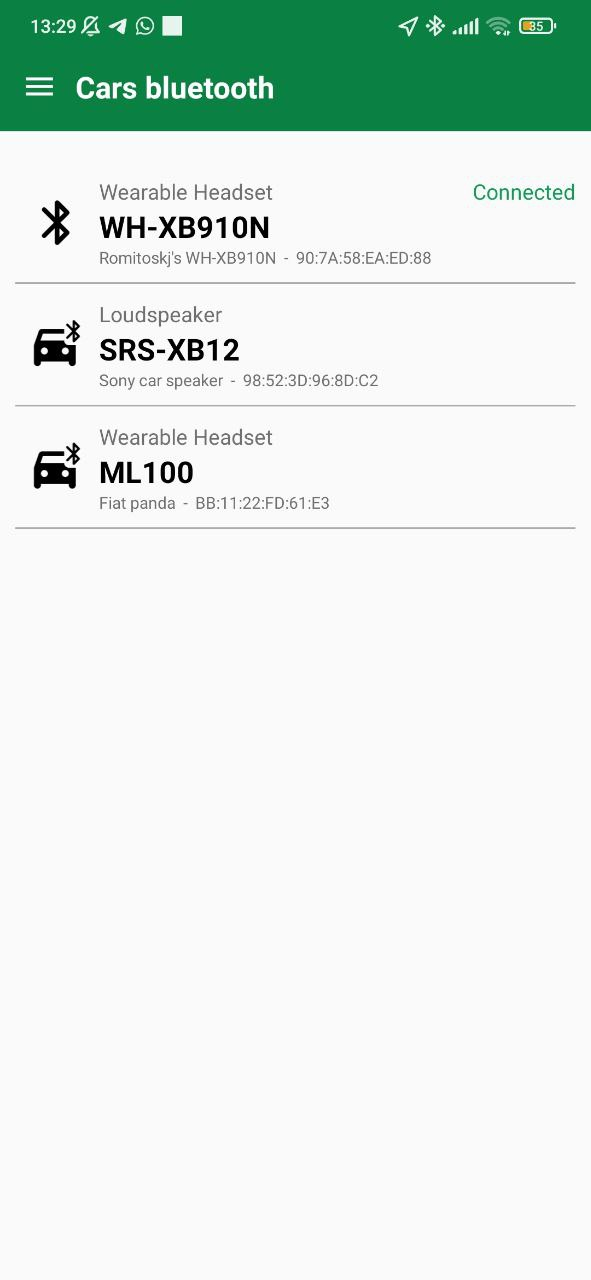
\includegraphics[width=0.9\linewidth]{images/bluetooth_activity.jpg}
    \caption{Interfaccia utente del sensore Bluetooth}
    \label{fig:bluetooth_activity}
\end{wrapfigure}
sia \textit{update} che \textit{collect} prendono in input un oggetto di tipo SensorData, il quale ha lo scopo di serializzare i dati relativi allo stato del sensore, come riportato nell'esempio qui sopra, per inviarli al server tramite la web API definita dal backend (paragrafo \ref{chap:sensorData}). Come per tutti i sensori, vengono serializzati la confidenza, l'azione compiuta dall'utente e il timestamp che indica il momento in cui è stato effettuato il calcolo. In aggiunta a ciò, nel campo data il sensore Bluetooth serializza il suo stato, indicando se il Bluetooth dello smartphone è acceso o meno e in caso affermativo riportando la lista dei dispositivi ad esso connessi. Inoltre per ogni dispositivo viene serializzato il nome, l'alias, la classe Bluetooth, il numero di connessioni effettuate con il dispositivo e un campo denominato \textit{is\_car} che indica se si tratti di un'automobile o meno.

\section{La presentazione dei dati}
Come per la prima applicazione sviluppata è stata creata un'interfaccia utente (visibile in figura \ref{fig:bluetooth_activity}) accessibile dal menu laterale di GeneroCity. Essa consente di visualizzare le auto salvate nella mappa \textit{cars} e i dispositivi connessi, il tutto in un unica lista ordinata in modo da avere i dispositivi connessi in alto e successivamente tutti gli altri ordinati in base al numero di connessioni effettuate. Di conseguenza, le automobili con più connessioni appariranno più in alto nella lista. Inoltre per ogni dispositivo è stata aggiunta un'icona che aiuta l'utente a distinguere se si tratta di un'auto o meno. Tutto ciò è stato implementato utilizzando un \textit{BluetoothDeviceAdapter} in maniera simile a quanto descritto nel paragrafo \ref{ref:presentation}. È stato quindi definito il metodo onDeviceUpdate in modo da fondere la lista dei dispositivi connessi e quella delle automobili, entrambe ottenute dal Controller, in un unica lista ordinata come descritto in precedenza. Questo metodo viene quindi registrato come listener del Controller in modo che, ogni volta che esso cambia stato, venga aggiornata l'interfaccia.

La definizione del BluetoothDeviceAdapter viene riportata qui sotto.
\begin{minted}[
framesep=2mm,
linenos,
bgcolor=LightGray,
breaklines
]{java}
BluetoothDeviceAdapter bluetoothDeviceAdapter = new BluetoothDeviceAdapter(this) {
    @Override
    public void updateDevices() {
        BluetoothController controller = BluetoothController.getInstance(
            BluetoothSensorActivity.this
            );

        Comparator<BluetoothDevice> deviceComparator = Comparator.comparing(
                        (BluetoothDevice bluetoothDevice) -> bluetoothDevice.isConnected(context),
                        Comparator.reverseOrder()
                )
                .thenComparing(BluetoothDevice::getConnectionCount, Comparator.reverseOrder())
                .thenComparing(BluetoothDevice::getLastConnection, Comparator.reverseOrder());

        devices = Stream.concat(controller.getCars().stream(), controller.getConnectedDevices().stream())  // merge cars and connected devices
                .distinct()  // remove duplicates
                .sorted(deviceComparator)  // sort by connection status, connection count and last connection
                .collect(Collectors.toList());

        notifyDataSetChanged();
    }
};
\end{minted}


\section{Il testing del sensore}
Sia durante lo sviluppo del sensore sia successivamente sono state effettuate delle prove con smartphone differenti e con alcuni modelli di macchine provviste di autoradio con Bluetooth, ciò allo scopo di verificare il corretto funzionamento del sensore Bluetooth. Le prove sono state effettuate tutte in sicurezza, poiché per questo sensore è necessario solamente instaurare una connessione tra l'auto e uno smartphone, senza la necessità di mettersi effettivamente alla guida. 

\subsection{L'identificazione di automobili}
I primi test che sono stati effettuati sono serviti a verificare il corretto funzionamento dell'algoritmo per identificazione di diversi tipi di dispositivi tramite le informazioni ricavate dal sensore Bluetooth. In particolare è stato importante controllare che le autovetture venissero rilevate come tali, indipendentemente se attraverso la classe Bluetooth o il nome del dispositivo.

Per effettuare questi test sono stati utilizzati diversi dispositivi allo scopo di verificarne il funzionamento su versioni di Android e hardware differenti. Gli smartphone utilizzati sono i seguenti: Xiaomi mi 9 Lite, OnePlus 6 e Xiaomi Note 11 Pro. Questi non hanno presentato differenze sostanziali durante la fase di testing. Inoltre, è stato possibile avere un riscontro dei risultati dei test attraverso l'interfaccia utente descritta precedentemente, visualizzando i log forniti dall'applicazione e analizzando i dati che sono stati inseriti nel database attraverso l'utilizzo della web API.

Prima di tutto sono stati effettuati test su diverse automobili con sistema Bluetooth integrato, per verificare che fosse indicata correttamente la classe Bluetooth relativa alle automobili (\texttt{BluetoothClass.Device.AUDIO\_VIDEO\_CAR\_AUDIO}). Dalle numerose vetture testate è emerso che, come precedentemente accennato, la classe del dispositivo ha sempre un identificativo più generico, ad esempio \texttt{handsfree} oppure \texttt{loudspeaker}. Per questo motivo si è deciso di implementare la rilevazione tramite nome o alias del dispositivo, dato che, anche se la classe è risultata generica, il nome dei sistemi integrati nelle auto ha sempre presentato informazioni sull'auto come il nome del modello o del produttore. Da qui si è presa la decisione di creare un piccolo database contenente il nome dei maggiori produttori di automobili, in modo da consentire l'identificazione tramite esso. Ciò permette anche di identificare dispositivi non integrati all'interno dell'auto, come casse Bluetooth o autoradio di terze parti, dato che essendo pensati per automobili presentano un alias coerente ("car", "auto", ecc.).

Dopo aver implementato le modifiche per effettuare l'identificazione tramite il nome, si sono eseguiti nuovamente dei test e si è osservato che il sensore è in grado di determinare automaticamente quando l'utente si connette ad un automobile.

\subsection{Verifica del valore di confidenza}
L'aspetto che si è voluto testare successivamente è l'aumento della confidenza coerentemente al numero di connessioni effettuate verso la stessa auto, allo scopo di rilevare con maggiore probabilità lo stato guida dell'utente. Infatti è importante che l'applicazione sia in grado di riconoscere quando l'utente si trova effettivamente alla guida e non sia un passeggero. Chiaramente il sensore Bluetooth da solo non può discernere questi due casi, quindi si è scelto di basarsi sul numero di connessioni  per inferire che, quando il dispositivo è connesso ad un auto utilizzata frequentemente, l'utente stia guidando.

Anzitutto si è testato un approccio lineare, ovvero aumentando la confidenza di un valore costante ogni qualvolta una nuova connessione con la stessa vettura fosse stata rilevata. Dai test è emerso che diverse situazioni, come l'utilizzo di servizi di car sharing o di uso sporadico di un automobile come passeggero, la confidenza restituita fosse troppo elevata portando a falsi positivi. Si è quindi deciso di utilizzare una funzione esponenziale in modo da incrementare leggermente la confidenza per le prime connessioni, mentre per un numero più elevato restituire una confidenza più alta. Questo approccio si è rivelato più affidabile nei successivi test.


\chapter{Conclusione}
Il lavoro descritto in questa tesi ha portato allo sviluppo e all'integrazione di un sensore Bluetooth all'interno dell'applicazione GeneroCity, con l'obiettivo di rilevare in modo affidabile quando un utente è alla guida di un veicolo. Questa soluzione, congiuntamente agli altri sensori, contribuisce a rendere l'esperienza degli utenti più sicura e comoda, riducendo la necessità di interazioni manuali durante la guida e facilitando la gestione intelligente dei parcheggi urbani. L'implementazione del sensore ha richiesto un'analisi approfondita delle API Android e la creazione di una strategia per la gestione delle connessioni Bluetooth. Infine il sensore sviluppato ha dimostrato di essere efficace nei test effettuati, rilevando correttamente la connessione a dispositivi compatibili con il contesto di guida, come le autoradio.


\section{Sviluppi futuri}
Per migliorare ulteriormente il sistema, sono attualmente in sviluppo presso il Gamification Lab modelli di machine learning per il calcolo dello stato di guida, così da sostituire in futuro la media pesata della confidenza dei vari sensori con algoritmi più sofisticati. Inoltre, sarebbe utile implementare un servizio esterno per verificare se il nome del dispositivo Bluetooth corrisponda a modelli di veicoli conosciuti, incrementando così l'accuratezza del riconoscimento. Questo servizio potrebbe essere implementato ad esempio attraverso un nuovo endpoint esposto dalla web API di GeneroCity, in questa maniera sia l'applicazione Android sia quella iOS potrebbero farne uso, in modo da effettuare in maniera centralizzata questa computazione.

L'utilizzo del sistema di rilevamento basato su sensori intelligenti come quello descritto in questa tesi per ottenere interazioni implicite rappresentano una direzione promettente per lo sviluppo di GeneroCity e più in generale nel campo della mobilità urbana.



\backmatter
\cleardoublepage

%\newpage
%\phantomsection
%\addcontentsline{toc}{chapter}{\indexname}
%\printindex

\newpage
\phantomsection
\addcontentsline{toc}{chapter}{\bibname}
\bibliography{bibiografia}

% %\begin{acknowledgments}
\chapter{Ringraziamenti}
SCRIVI QUI I RINGRAZIAMENTI 
%\end{acknowledgments}

\end{document}